\documentclass[11pt,a4paper]{article}
\usepackage[margin=23mm]{geometry}
\usepackage{tikz}
\usetikzlibrary{positioning,arrows.meta}
\title{HyMeKo, XML, YAML and JSON: equivalent-data parsing comparison}
\date{Created-at: 2026-09-07 20:33 +02:00}
\begin{document}\maketitle
\paragraph{Owner and authority.} Parser owns the frontend benchmark. User explicitly
requested an exhaustive comparison with XML, YAML and JSON. Only benchmark/test
dependencies and clients change; production parser and Core are unchanged. Parser
HEAD equals freshly fetched origin/master 284c490, clean at task start. Core's
earlier uncommitted optimizations remain untouched. The provider map and actual
parser manifest confirm the owner. No local Parser CORE.YAML exists; no production
dependency is added, and this request authorizes the required isolated test libraries.
\paragraph{Scope and ETA.} Approximately 40 minutes: helpers/build/tests 12,
production-scale smoke 3, two measured rounds 20, analysis/report 5. Five patterns
(flat, linked, Unicode, long text, nested), four logical-node scales
(100, 1000, 10000, 50000), four formats and three boundaries (serialize, parse
document, decode common records): 240 cells per round, two rounds. Ten post-warmup
samples per cell using Criterion flat sampling. This is a broad declared corpus,
not proof for all inputs or all implementations of each language.
\paragraph{Representation and equivalence.} One deterministic owned record tree:
unique identifier, finite numeric value, text, signed weighted links and children.
Generate each case once, serialize all formats, and compare every decoded record
against the generator before timing. Fixture manifest records bytes, hashes, counts,
depth and generation/encoding diagnostic times. Library-native AST/DOM representations
differ and must be labelled. Decode returns the same owned records. This is not
HyMeKo semantic IR compilation or execution; no unfair comparison against hashing
or reference resolution. Both bytes/s and logical records/s accompany latency.
\paragraph{Libraries.} Existing HyMeKo SIMD-dispatched parser; serde\_json;
roxmltree for XML DOM, quick-xml for XML serialization/typed decoding;
serde-saphyr for YAML generic values/typed decoding. Record exact lockfile versions
and settings. Keep default parser limits and report any rejected case. No CUDA,
QEMU or Python parser timings mixed into this same-host Rust comparison.
\paragraph{Affected files.} Parser Cargo.toml and Cargo.lock (dev dependencies and
bench registration), benches/parser\_bench.rs (assert successful parses),
benches/format\_bench.rs, benches/formats.rs (or a cohesive helper directory if
needed), tests/format\_comparison.rs, scripts/format\_campaign.py, this four-format
plan and reports/2026-09-07-format-comparison.md plus its numerical/plot evidence.
Existing Core memory harness is reused, not copied; no production API change.
\paragraph{Tests and experiment.} Round-trip all shapes and sizes before scheduling;
tests independently assert record fields, signs/weights, Unicode/escapes, nesting,
empty values, malformed/truncated sources and semantic mismatch detection. Original
HyMeKo generators must parse successfully instead of timing an unchecked Result.
Run Parser tests and applicable formatting/lint. Preflight new helpers. A maximum-size
smoke precedes the matrix. Each parse/decode process loads only its resident input;
serialization processes load the common record tree. Generation and I/O are outside
timers. Exclude final destruction from phase timers. Verify binary and fixture hashes.
\paragraph{Budgets and observability.} At most 16 GiB observed peak resident memory
and 180 seconds per cell, enforced by the campaign monitor; VAS is not capped.
Fresh subprocess per cell, sequential on a quiet host. Capture growing logs, exit
status, CPU/wall/progress and peak memory; resume only verified completed cells from
the same binary and fixtures. Failure is recorded, never a speed result. Large
strings/deep nesting can hit library limits; record the cause, do not silently shrink
or disable guards. Report median, inclusive IQR, worst and all raw Criterion samples.
\paragraph{Output and rollback.} A readable report, raw JSON and modern interactive
plots plus an exportable figure. State library/phase, input semantics, sample count,
platform and limitations on every plot. No universal format ranking. Revert only
named benchmark changes if invalid; retain diagnostic evidence and user changes.
\paragraph{Correctness finding, 20:39.} The independent mixed escape/Unicode
round-trip fails on the actual parser: lex\_string casts UTF-8 bytes to characters
on its escape path. Extend the scope narrowly to src/lexer/common.rs: accumulate
decoded bytes and validate UTF-8 once when constructing the owned string. Preserve
the existing ASCII escape and unknown-escape behavior. No dependency or public API
change. Freeze the failure and test scalar/SSE2/AVX2 before measuring; record the
uncommitted correction in benchmark provenance. This repairs an observed correctness
defect discovered by the requested comparison, not a speculative speed change.
\paragraph{Budget finding, 20:47.} The YAML default rejects the flat 50k fixture
at 250001 parser nodes (limit 250000). Record default-policy rejection per fixture,
and use a separately disclosed finite corpus budget of 5 million YAML nodes and
10 million events for measured YAML cells. Keep all other YAML limits, including
depth 64 and scalar bytes 64 MiB. Never time default rejections as successful parses.
This explicit policy permits the same large workload without disabling guards.
\paragraph{Publication, 20:56.} Reuse the existing Next.js Observatory and Plotly
renderer/HUD on Amaterasu; add a Matched formats tab and a typed observation adapter.
Affected web files: src/app/observatory.tsx, src/app/formats.tsx,
src/lib/formats.ts, src/app/globals.css, tests/format.test.mjs,
tests/browser.mjs, public/formats/*, tools/plot\_reports.py and compose.yaml.
The web checkout is local-only (no remotes), main caca3a5, with prior authorized
UI changes preserved. Parser owns numerical aggregation in scripts/format\_report.py;
the web consumes verified artifacts only. Reuse its exporter for SVG. Validate
same-source values, complete coverage, hover/pin, 2D/3D axes and mobile layout;
then build and deploy with rollback to the existing purple-platforms image.
ETA from measured initial cells: campaign completes around 21:10, report and
browser-verified publication around 21:20. No runtime algorithm or Core change.
\paragraph{Stability follow-up, 21:10.} All 480 cells succeeded in 836.6 seconds,
but 53 of 240 paired observations differ by more than 20 percent between rounds.
Balanced power and hybrid CPU scheduling are candidate explanations, not established
causes. Add an optional affinity mask and shared-fixture path to the existing runner.
Run nested/long-text 50k, all four formats and all three phases, two rounds (48 cells)
on logical CPU 0. Preserve the original campaign and publish this as a separate
sensitivity check; do not selectively replace slow values. Verify child affinity.
Expected 2--3 minutes, same 16 GiB/180 s budgets; source/binary unchanged.
\paragraph{Browser finding, 21:25.} A direct Matched formats load fetches data
asynchronously; the shared HUD resolves its dock before that element exists and
keeps a floating popup. Fix the existing ObservationProvider lifecycle to observe
late dock insertion and detach the observer on resolution/unmount. Add an optional
dataset guide URL to Observation so format points link to their own guide. Let the
existing Plotly renderer preserve a caller-supplied legend title. Additional web
files: src/app/observation.tsx, src/lib/observations.ts, src/app/plot.tsx. Verify
direct-load desktop docking, mobile floating fallback, cleanup and existing views.
\paragraph{Optimization continuation, Created-at: 2026-09-08 02:17 +02:00.}
User requests further optimization. ETA 40 minutes: symbolized profile/build 10,
focused implementation and tests 15, matched before/after experiments and report 15.
Parser owns this work; Core protected items: empty. Fresh Parser fetch matched
origin/master 284c490; preserve all previous campaign edits. Reuse this plan,
format benchmark, campaign runner and report; keep new evidence under
reports/format-comparison/optimization. Before changes preserve source and matching
executable/PDB. Profile actual native AST parsing on linked and long-text 50k
fixtures with samply; no adapter costs attributed to Core. Candidate causes:
grammar temporary list allocation, lexer repeated scans, generated parser stack
movement. Select only a demonstrated hot path. Possible affected production files:
src/hymeko.lalrpop and src/lexer/common.rs or simd.rs; no public API, accepted
language, AST shape or dependency change. Extend tests/format\_comparison.rs for
boundaries, malformed input, long lists, nesting and SIMD parity. Extend existing
runner only if needed for focused format selection. Unchanged fixtures/hashes,
fixed CPU 0, identical release/debug settings for both binaries, at least two
independent rounds of ten post-warmup samples; reverse A/B order and investigate
spread above 10 percent. Smoke at 50k before focused matrix. Preserve 16 GiB RSS
and 180-second process guard; latency/memory regression above 10 percent blocks
acceptance until isolated. Profile includes destruction and harness: separate
phase times remain the speed evidence. No claimed Core IR/runtime or cross-platform
speedup without separate measurement. Roll back only this continuation's production
hunks if no demonstrated benefit; keep original Unicode fix and baseline evidence.
Emit raw values, median/IQR/worst, matching provenance, profile and comparison figure.

\paragraph{String scanning continuation, Created-at: 2026-09-08 02:50 +02:00.}
User authorizes the next measured Parser hotspot. ETA 25 minutes: implementation
and semantic controls 8, paired measurements and profile 8, gates/report 9.
Reuse final.exe/final-source.zip and the long-text CPU profile from the preceding
optimization as baseline; do not discard the grammar optimization. Fresh fetch:
Parser master and origin/master 284c490, zero divergence; previous dirty files kept.
Owner: Parser. CORE.YAML items touched: empty. No new dependencies or public APIs.
Affected files: src/lexer/common.rs, tests/format\_comparison.rs, this plan bundle,
existing format-comparison report, generated optimization/string-scan evidence.
Add one private pure helper to skip ordinary string bytes using safe eight-byte
loads and a word-parallel zero-byte test for quote/backslash; scalar search finds
the exact delimiter and handles tails. Preserve source-borrowed strings, UTF-8
escape decoding, source spans, unterminated/invalid-UTF8 errors and lexer position
on failure. No new unsafe code, CPU feature assumption, global state or allocation.
Test every byte/lane and short tail against an independent scalar search, delimiter
pairs and high-bit bytes; integration tests at block boundaries, long strings,
Unicode, known/unknown escapes, malformed endings and all lexer tiers. Run on
baseline and candidate before timing. The existing 50k long-text profile places
lex\_string in 26.07 percent of parse samples; this is measured, not conjecture.
Smoke 50k then focused native-AST paired A/B for all five patterns, 100/10000/50000
records where needed, ten warm samples per process and two independent rounds
with reversed case/variant order. Same binary flags and CPU 0 affinity; existing
16 GiB and 180-second process guards. A latency or repeated-memory regression over
10 percent requires investigation; discard an unhelpful candidate. Record sample
spread, do not replace slow values. Profile final long-text path separately from
timings. Preserve exact binaries/PDB/source, numerical and plotted output. Core
IR/runtime and downstream deployment remain separate unmeasured boundaries.
Rollback only this continuation's named changes; preserve the earlier UTF-8 repair
and LALRPOP grammar improvements.

\paragraph{AST list continuation, Created-at: 2026-09-08 03:36 +02:00.}
ETA 25 minutes: bounded list change and semantic tests 8, paired JSON controls
and profile 10, gates/report 7. Parser master 284c490 matches freshly fetched
origin/master; preserve all earlier dirty changes. Owner Parser, protected Core
items empty, no dependency or public type/API change. User requests JSON parity
before continuing the original CUDA plan. Treat that condition as unfulfilled
until matched parsing results support it; record DOM/AST and typed decoding
separately and do not substitute a single favorable workload for the whole suite.
Current long-text profile attributes 23.5 percent of parse samples to HyperItem
vector growth. Generated HyperItem+ seeds vec![first], so every two-item body
grows immediately. Hypotheses: tiny-body reallocations versus large-list growth.
Introduce private HyperItems/HyperItemsMany grammar rules: empty and singleton
keep exact allocation behavior; the first pair is allocated together, and later
items append normally. This targets two-item bodies without oversizing singletons.
No input pre-scan, guessed byte-to-node capacity, or parallel grammar/parser.
Affected production file src/hymeko.lalrpop; extend tests/format\_comparison.rs
with empty/single/pair/large mixed node-edge-arc sequences and malformed endings.
Extend benches/format\_bench.rs only if an untimed capacity/shape diagnostic is
needed. Reuse scripts/format\_campaign.py and format\_report.py; evidence in
optimization/item-list. Preserve before/after binary, PDB and exact source.
Smoke max-scale flat/linked/long-text before timed matrix: all five patterns,
native AST and common records at 50k, two fresh rounds with ten samples, CPU 0,
rotated baseline/candidate/JSON order. Check small and singleton-heavy sources
separately for memory regressions; use existing fixture/semantic oracles.
Every process retains 16 GiB observed working-set and 180-second guards.
Investigate latency or memory regression over 10 percent. Capture candidate
profile on long-text 50k, compare inclusive stacks without summing nested shares.
If the targeted change fails, restore only this stage's production changes and
retain evidence. No GPU work while latency samples run. CUDA follow-up reuses
the existing Phase 6 feasibility and platform-audit plans when the user's
parser condition is met; no new backend or dependency is implied by this step.

\paragraph{Remaining frontend costs, Created-at: 2026-09-08 04:00 +02:00.}
ETA 25 minutes: linked/Unicode profiles 5, isolated implementation and tests 8,
paired three-way measurements 7, gates/report 5. Fresh Parser fetch matched
master/origin 284c490 with existing changes preserved. Owner Parser; protected
Core items empty; no dependency, public API or new unsafe code. Preserve current
item-list executable/PDB and source as baseline under optimization/frontend.
Profile linked and Unicode native AST at 50k before choosing changes. Distinguish
grammar reduction/stack movement, numeric conversion, allocation and string escape
decoding. Candidate files src/hymeko.lalrpop, src/lexer/common.rs or simd.rs;
existing tests/format\_comparison.rs must cover every touched path and preserve
values, order, borrowing, Unicode and malformed-input diagnostics. No manual edits
to generated parser source. Build before code mutation only after this plan
compiles. Use the existing runner and identical hashed fixtures: baseline/new/JSON
at 50k, both AST/DOM and common records, two adjacent rotated process rounds,
ten samples, CPU 0. Smoke largest cases first; check small cases if a fast path
changes. Preserve 180-second and 16-GiB guards. Investigate regressions above ten
percent, retain failures/variance, profile speedups and roll back unhelpful hunks.
Existing optional wrappers and item-list optimizations remain. Report exact
source/binary provenance, raw samples, memory, SVG/PDF plot and residual JSON gap.
CUDA remains conditional on the parser milestone; do not infer it from one case.
\paragraph{Load investigation, 2026-09-08 04:09 +02:00.}
CPU-0 campaign stopped after broad transient slowdowns and a 99-percent host
load observation. Preserve completed raw cells as contaminated diagnostics;
do not selectively keep favorable samples. External browser/download processes
were observed and are not modified. Three follow-up per-CPU observations show
CPU 2 idle while CPU 0 remains busy. Run a separate complete paired control on
logical CPU 2 (affinity mask 4), all variants equally. Record the CPU-selection
observations and inspect process-round spread before acceptance. This is still
a shared desktop, not a claim of OS isolation. CPU-0 and CPU-2 timings stay separate.
\paragraph{Native Linux control, 2026-09-08 04:16 +02:00.}
The CPU-2 run also contains multi-fold drift; keep both Windows campaigns as
diagnostics, not acceptance evidence. Amaterasu has low observed load, 32 GiB RAM
and installed Rust 1.97.1. Additional ETA 15--20 minutes for transfer/build, native
paired controls and report. Use archived before/after sources and the identical
hashed fixtures, explicit cargo +1.97.1, matching release/debug flags, and no
cross-platform ratio. Artifact directory /tmp/hymeko-parser-frontend-20260908;
no new Git checkout or branch. Reuse Graph ProcessRunner for the Linux 50-ms
VmHWM sampling and 180-second/16-GiB guards. Extend existing Parser Campaign with
an optional checked invocation adapter; default Windows behavior unchanged.
Additional files scripts/format\_campaign.py and scripts/test\_format\_report.py;
test adapter forwarding/resource rejection. No production dependency changes.
The temporary Linux invocation only maps the existing monitor's output into the
existing campaign schema. Preserve its exact source and Graph monitor hash.
All five 50k inputs, both phases, baseline/new/JSON in adjacent reversed rounds;
same CPU affinity for every variant. Candidate profile remains separately captured.
\paragraph{Owned-record diagnosis, 2026-09-08 12:00 +02:00.}
Owner: Parser benchmark adapter only; protected Core items empty. ETA 20 minutes:
baseline extraction and staged diagnosis 6, ownership change and tests 5,
matched native measurements 4, gates and report 5. Fresh fetch matched 284c490,
zero divergence; preserve all existing work. Extend benches/formats/adapters.rs,
benches/format\_bench.rs, tests/format\_comparison.rs and this plan/report bundle.
Reuse Campaign's native invocation adapter, existing fixtures and Graph monitor.
No dependencies, unsafe code, grammar or production API changes. Expose the
existing benchmark Dataset projection for a pre-parsed-input measurement; retain
its baseline source and executable before replacing borrowed traversal with
consuming traversal and Cow::into\_owned. Baseline diagnoses parse, borrowed
projection and AST destruction separately. Candidate measures consuming conversion
(including interleaved AST cleanup); do not compare that stage as pure projection.
Both retain the identical full decode\_records timing boundary and final-output
destruction exclusion. Add dedicated drop\_ast and consume\_ast benchmark phases;
baseline-only project\_records is retained in the archived baseline, not as a
duplicate production converter. Exercise new branches through Criterion smoke.
Tests: exact records, negative zero, empty/nested/linked inputs, malformed record
fields and ownership transfer of already-owned strings, including empty strings.
Capture baseline CPU attribution if samply is available; keep prior profiler
failure evidence explicit otherwise, and do not invent a hotspot share.
Native Amaterasu: inspect load first, CPU 2, Rust 1.97.1, same source/fixture hashes,
two reversed rounds, ten samples each. First stage smokes at 50k linked/long text;
full decode A/B/JSON on five 50k patterns, focused small-case regression controls.
180-second process / observed 16-GiB cap; investigate greater-than-ten-percent
regressions and uncertainty. Retain source snapshots under optimization/ownership;
rollback only this stage's adapter and benchmark hunks if unhelpful. Record
complete raw samples, IQR, peak RSS, source delta, checks and SVG/PDF plot.
\paragraph{Persistent regression checks, 2026-09-08 12:49 +02:00.}
ETA 20 minutes: gate and independent tests 9, native scale controls 4, gates and
report/plot 7. Owner Parser; Core items empty; no dependency or algorithm changes.
Fresh fetch matched origin/master 284c490, divergence zero. Extend existing
scripts/format\_report.py with a comparative gate and CLI, format\_campaign.py
with host identity, scripts/test\_format\_report.py with invalid-input, threshold,
CLI and generated monotonicity/scale laws using already-installed Hypothesis.
Extend tests/format\_comparison.rs with nested owned/borrowed buffer checks.
Before accepting, require same host/platform/machine/CPU affinity, phase boundary,
fixture bytes/hash, matching complete two-round matrices, ten positive finite
samples per round, successful process exits and valid observed resource budgets.
Recompute statistics from raw samples; do not trust saved summary medians.
Default time/peak regression and round drift bounds ten percent. Distinguish pass,
regression, invalid evidence and inconclusive drift; every non-pass exits nonzero.
Do not mark noisy evidence green or manufacture absent historical host metadata.
Expose a reusable local/CI command; no CI provider/runner is configured in this
checkout, so do not claim an active remote pipeline. Mutation tests must prove
the gate rejects a real slowdown and restored string copying fails the pointer test.
Reuse immutable ownership before/after binaries and same native monitor; new
10k/50k five-pattern full decode controls plus matched JSON, two reversed rounds,
production-scale smokes first. Preserve 180-second / observed 16-GiB guards,
record CPU profiles already establishing current costs, and do not rerun unchanged
Rust builds merely for measurements. Reuse existing plotter and report; store new
raw evidence under optimization/regression-checks. Roll back only new hunks if
gates fail; preserve all prior work. No new production parser or direct-AST bypass
is attempted without its own semantic design and evidence.
\paragraph{PERF-2 AST construction, Created-at: 2026-09-09 19:47 +02:00.}
Owner Parser; Core protected items empty. ETA 30--40 minutes: grammar candidate
and controls 10, matched measurements/profile 15, report/publication 10.
Base 0019eb0 equals freshly fetched GitHub and LAN course branches. Reuse the
course integration branch in its retired worktree path to keep the published
control separate from the original dirty master checkout and its historical edits.
Prior consuming-record linked profile: 4329/9264 samples include LR reduction;
6970 include parsing. Test the hypothesis that declaration-to-item reductions move
large AST values unnecessarily. Inline declaration constructors into their existing
consumers in the single LALRPOP grammar; no generated-source edits, second parser,
new dependency or public API. Candidate files src/hymeko.lalrpop and existing
 tests/format\_comparison.rs; this plan bundle and the existing report. Retain or
roll back based on same-host controls; do not claim AST-free decoding from this.
Before candidate code, save published executable/PDB and grammar; strengthen
semantic/invalid-input tests on baseline, then candidate. Preserve node/edge/arc
order, tags, signed paths, nested values, UTF-8 and exact diagnostics. Measure
50k records in all five patterns, AST and owned records separately, same harness,
release debug=1, CPU 0, two reversed rounds, ten post-warmup samples. Run large
smokes first; memory cap 16 GiB and 180 seconds per process through existing runner.
Generation/I/O/final-output drop excluded as before. JSON typed/DOM controls are
separate boundaries. Investigate over-10-percent regressions; inconclusive gates
are not passes. Capture a matching candidate profile for a greater-than-10-percent
speed claim. Code-size growth and small-input controls are explicit risks.
Record raw samples, median/IQR/worst, peak RSS, source/binary hashes and SVG/PDF.
If unhelpful, restore only this candidate's hunks; retain evidence and the original
PERF-1 release. No consumer pin or SDK publication without an accepted provider.
\paragraph{PERF-2 generator finding, 19:53.}
Stop all-three-constructor candidate after 167 seconds in LALRPOP generation;
last observed memory 54.2 MiB, CPU 132.8 seconds. No executable or speed claim.
Inlining multiple declaration alternatives compounds at the existing first-pair
list production. Narrow the same hypothesis to the single HyperArc constructor;
record rejected patch and build evidence. The accepted-language/diagnostic oracle
is fixed from the published baseline, never updated to accommodate the candidate.
\paragraph{PERF-2 typed output construction, Created-at: 20:04 +02:00.}
Continue the authorized PERF-2 after rejecting the reduction-only probe. ETA
45 minutes: API/grammar and parity 20, focused A/B and controls 15, integration
and archival 10. Parser owns a generic OutputBuilder contract with native AST
and owned-record implementations. Keep a single LALRPOP grammar. Generalize
Description and node/edge bodies with a default item type, preserving existing
source signatures through default type parameters. Add an explicit builder entry
point; retain existing parse entrypoints and DescriptionParser/QueryVarParser
facades, including token conversion and exact parse errors. No new dependencies,
unsafe code or protected Core implementation changes. Additional files:
src/builder.rs, src/lib.rs, src/ast.rs, src/hymeko.lalrpop,
benches/formats/adapters.rs, benches/format\_bench.rs and existing format tests.
Builders receive every syntactic construct; native AST is the compatibility
implementation. Header types and value/reference syntax remain canonical. Callback
side effects before a later syntax error are documented, never transactional by
implication. Owned-record semantic errors are stored and returned only after
successful syntax parsing, preserving existing error precedence and field order.
Keep full AST projection as an independent test/measurement oracle; default typed
decode may switch only after parity and measured improvement. Test headers,
all node forms, nested records, reserved field names at roots/inside blocks,
malformed records, ownership transfer, lexer errors and the existing frozen full
AST/error digest. All native tests, Clippy, touched formatting, public API checks;
measure original default AST and direct records separately using unchanged fixtures,
runner/caps, same host and at least two rounds. Preserve 1000/50000 controls and
code size. No claim of Core IR or browser speed before consumer integration.
Rollback all builder production hunks on unresolved compatibility or regressions;
retain controls and evidence. Expected memory remains below prior 349 MiB timed
peak by a wide margin; 16-GiB / 180-second process guards still apply.
\paragraph{Typed-output native control, 20:14.}
Windows: 72 cells complete; one stable linked-record gate passes, eleven cases
are inconclusive. Large owned-record pooled medians improve 21--26 percent;
native AST no universal win. Small linked memory is unstable and needs a
native control. Amaterasu observed load 0.15/0.09/0.06. Use /tmp/hymeko-parser-typed-output-20260909
with exact 0019eb0 and candidate source archives, Rust 1.97.1, release debug=1,
CPU 2 for all variants, existing fixtures and Graph ProcessRunner. Reuse the old
build cache but retain independent executable/source pairs. Two rounds on the
same 1000/50000 cases, 16-GiB / 180-second guards. Capture separate Windows samply
profiles on linked/Unicode before and after; no latency measurements alongside
profiling or builds on that host. Additional ETA 15--20 minutes.
\paragraph{API inference regression, 20:26.}
A new compile regression proves that adding a default Item parameter to the
public Description breaks an existing unannotated empty struct literal (E0282).
Restore src/ast.rs exactly. OutputBuilder will use construction-input types in
its own module: DescriptionInput (name, existing HeaderBlock, built items), shared
DeclarationBody plus NodeInput/EdgeInput aliases using the existing annotation
wrapper. AstBuilder moves these fields into the original AST types without
allocation. This preserves caller inference and Debug shape and keeps construction
inputs separate from the canonical native AST; no second semantic IR. Re-run
native/owned controls after this representation boundary correction. Retained
owned-buffer diagnostic at 1000 records is lower for the direct builder in all
five patterns; freeze that allocation-capacity bound as an additional test.
\paragraph{Final verification and collector correction, 21:06.}
The final API preserves the original AST and lexer source. A Windows deep-path
collector failure exposed a silent glob omission after 18 accepted cells; extend
the existing Campaign path handling for local and UNC paths, add real deep-path
and mocked UNC regressions, retain the orphaned raw data and resume by hash.
Final added tooling scope: scripts/format\_campaign.py, scripts/format\_report.py,
scripts/test\_format\_report.py and generated SYMBOLS.md. Final production scope
excludes src/ast.rs and benches/format\_bench.rs. Core changes strategy docs only;
protected items remain empty. Both 72-cell final controls completed. Linux flat
and Unicode owned medians improve 10--11 percent; linked remains inconclusive,
long-text is 2.33 percent slower, AST has no measured gain. JSON remains faster.
All 123 Parser tests, 2 doctests, 11 Python methods, 20 large round trips and
457 Core tests plus 7 doctests pass. WASM library compile-check passes.
Publication retains the unchanged Core/SDK pins; no default-branch merge.


\paragraph{JSON catch-up continuation, 2026-09-10 03:53 +02:00.}
Created-at: 2026-09-10T03:53:00+02:00. ETA: 25 minutes for the first candidate
and targeted correctness checks; the user explicitly authorized targeted JSON benchmarks and profiling at 03:58.
Owner: Parser. Reuse parser-course-release, fast-forwarded to published master
f116285 after fetching origin and github; preserve its existing .gitignore delta
and the separate dirty parser checkout. No new worktree or Core source change.
The archived compatible Unicode after-profile attributes 1939/9269 inclusive
samples to lex\_string. Its escaped path scans once for the closing delimiter,
then copies every byte separately. Reuse string\_prefix\_len for bulk copying
ordinary runs and remember the first escape to avoid scanning the prefix twice.
Preserve borrowed plain strings, owned escaped strings, unknown escapes, UTF-8,
error text/offset and lexer position. Add a character-based decoding oracle over
boundary lengths and escaped Unicode; run exact lexer and frozen diagnostic tests.
Authorized scope: current Parser versus JSON, baseline/candidate on identical
fixtures; 50k Unicode first, then affected and plain-string controls. Reuse
Campaign and its 180-second process timeout / 16-GiB observed-memory guard.
Two reversed rounds, ten Criterion samples after warmup. Profile separately
from timed cells. Preserve source, binary/PDB and raw evidence in ignored reports.
Performance acceptance is conditional on the evidence recorded below.
Seven targeted correctness tests pass, including a character-based escape oracle,
unterminated-string cursor checks, all available lexer backends, frozen parser
diagnostics and four-format record parity. Clippy with warnings denied passes;
the additional cognitive-complexity lint flags generated LALRPOP code only
(generated code is exempt). Measurement authorization received; results follow in the existing report.


\paragraph{Constructor boundary probe, 2026-09-10 04:19 +02:00.}
ETA: 15 minutes; Parser grammar only, no Core item/API/lexer change beyond the
separately retained escaped-run candidate. Current symbolized Unicode profiles
still concentrate samples in item-list reduction and output construction.
The earlier rejected all-constructor inline probe compounded alternatives through
inline HyperItem and the first-pair list production. Keep HyperItem as an explicit
nonterminal while inlining NodeDecl, EdgeDecl and HyperArc into it: preserve the
compact first-pair list and callback ordering, eliminate temporary constructor
values without their cross-product at every list site. Bound generation to 120 s.
Accept only if the frozen AST/error digest and builder contracts pass, generation
stays bounded, and matched native full-record plus AST controls justify the change.
Otherwise restore only this grammar delta; the escaped-run evidence remains.


\paragraph{Measured checkpoint, 2026-09-10 04:23 +02:00.}
Retain escaped-run copying only. Native paired 50k Unicode full-record decoding:
39.478 to 35.631 ms median (9.75 percent lower); five large-input timing/RSS gates
pass. The full seven-case gate retains a small-input RSS regression flag and one
inconclusive small-input row. Investigating that flag: identical-binary A/A gives
19.49 percent peak spread; five post-warmup continuous-workload pairs give median
5.914 vs 5.855 MiB. Do not relabel the original gate or claim all-green memory.
Windows timings are inconclusive. Matched symbolized Windows CPU traces show
lex\_string in 662/3575 vs 289/1740 inclusive decode samples; these are supporting
sampled indicators, not additive time measurements. JSON parity remains unmet.
The constructor-boundary probe generates promptly and preserves the frozen oracle,
but gives only 1.02 percent Unicode decode improvement and 4.23 percent flat decode
regression. Restore its grammar delta; retain its source/binary/raw evidence.
Also separate the existing comparative retained-storage profile from correctness:
it is ignored by default and both benchmark targets declare test=false. Normal
selection demonstrably skips the profile; explicit ignored/exact invocation passes.
No Core, Graph, Transformation or consumer pins change in this Parser-only step.


\paragraph{Vector string delimiter probe, 2026-09-10 20:50 +02:00.}
ETA: 25 minutes: targeted tests, incremental native builds, paired full-record
controls and evidence archival. Owner: Parser; reuse the synchronized existing
checkout at 02ae74c and Amaterasu 192.168.1.228. Core protected items: none.
Options from existing profiles: LR reduction/list movement (largest share,
constructor inlining already rejected), escaped-string allocations/validation,
and plain delimiter scanning. Probe the last with the smallest portable change:
use baseline x86-64 SSE2 to scan sixteen bytes at a time inside the existing
string\_prefix\_len; preserve the existing eight-byte/tail fallback elsewhere.
No runtime feature dispatch, dependency, public API or grammar change.
Discovery: common.rs owns the only string delimiter scanner; simd.rs contains
whitespace/identifier kernels, no string kernel. Existing candidate profile
attributes 289/1740 inclusive decode samples to lex\_string and 27 to its scan.
This is a bounded hypothesis, not a promised end-to-end gain. No new scaffold.
Scope: src/lexer/common.rs, its existing correctness tests, existing plan/report.
Every vector read must be bounded by a complete sixteen-byte slice; arbitrary
UTF-8 bytes are opaque, quotes and escapes remain byte delimiters. Test every
vector/tail alignment against an independent scalar oracle and retain existing
escape/error cursor tests plus frozen AST diagnostics and builder parity.
Compare the prior escaped-run candidate against this change on identical native
fixtures: long text first, then Unicode/plain/linked/nested and small controls.
Two reversed rounds, ten warmed Criterion samples, CPU 2, 180-second timeout and
16-GiB observed cap. Timing excludes fixture creation and final output drop.
Rollback only the scanner delta if no stable benefit or any unexplained regression;
preserve unrelated .gitignore and generated files. Reuse canonical campaign,
report and provider archive tool; no new worktree. Profile separately if needed.


\paragraph{Vector scan outcome, 2026-09-10 20:57 +02:00.}
Retain for review: matched native long text 61.069 to 56.853 ms (6.90 percent),
Unicode 35.785 to 34.220 ms (4.37 percent); focus timing/RSS gates pass.
Controls retain a small Unicode RSS regression flag (7.012 to 8.125 MiB),
two inconclusive cases and a 5.48-percent nested latency increase within budget.
Five continuous-workload memory pairs give 6.082 to 6.148 MiB median; same-binary
A/A is inconclusive. These investigate but do not erase the original flag.
Ten targeted correctness tests pass on Windows, five scanner tests on Linux;
Clippy and WASM compile pass. No default-branch merge or consumer pin change.
Next opportunity: intermediate list/value construction, based on existing
reduction and Vec-push profiles; no new grammar or API redesign implemented.


\paragraph{List wrapper continuation, 2026-09-10 21:04 +02:00.}
ETA: 20 minutes. Freshly fetched Parser branch equals both remote heads at
686ce81. Owner: Parser; Core protected items and dependency changes: none.
Existing profiles identify ValueList/SignedRefList construction and generated
reductions as hot paths. Separated already accumulates directly, but each completed
value/reference vector still crosses a forwarding LR nonterminal. Inline only
ValueList and SignedRefList into their existing callers; retain Separated and all
public AST/builder types, order, trailing-comma and syntax-error behavior.
This eliminates representation forwarding, not the owned output allocations;
no allocation-count reduction is claimed without measurement. Constructor
inlining is a separate rejected candidate and is not repeated.
Discovery: these two rules are canonical in hymeko.lalrpop; existing list/annotation
and frozen AST/diagnostic tests cover them. Extend existing list cases with lengths
around growth boundaries and larger lists. Source changes: two private grammar
annotations/comments, targeted test expansion, existing plan/report. No new API.
Run the expanded tests on the current baseline first, then the candidate; cap
code generation/build at 120 seconds. Native A/B against 686ce81 uses identical
inputs and existing campaign, CPU 2, two reversed rounds, ten warmed samples,
180-second process limit and 16-GiB observed cap. Start linked full decoding,
then flat/Unicode; broaden to relevant control cases only if useful. Restore
only the grammar delta if benefit is absent or a regression remains unexplained.


\paragraph{Owned link-buffer probe, 2026-09-10 21:07 +02:00.}
Reject list-wrapper fusion: linked latency improves only 0.97 percent while its
process RSS rises 11.32 percent; Unicode is inconclusive due baseline round drift.
Restore the exact pre-probe grammar. Keep the expanded independent correctness cases.
Next owner: the benchmark's existing typed RecordBuilder adapter, not the production
parser grammar or Core. Completed Link vectors are copied into empty vectors twice,
at arc-to-edge and edge-to-record boundaries. Existing linked profiles contain
allocation/vector movement; source inspection identifies these avoidable copies.
Preserve source order, first-error precedence and retained output capacity. Transfer
the first suitable owned buffer; append subsequent groups normally. Do not retain
an oversized incoming allocation merely to make the timing look better.
Scope: benches/formats/adapters.rs and tests/format\_comparison.rs; no public API,
new dependency or production parser change. A deterministic pointer/capacity test
must fail on the original adapter and pass after the change. Existing builder/AST
parity and explicit retained-storage profile remain controls. Measure linked native
owned decoding against 686ce81, then other cases if useful; same caps/harness.
This can improve the measured consumer; it is not a universal parser speed claim.


\paragraph{List/buffer outcome, 2026-09-10 21:13 +02:00.}
Grammar probe rejected and restored: linked RSS +11.32 percent for less than
one-percent time benefit. Retain the benchmark RecordBuilder ownership change
only. Pointer/capacity test fails before and passes after; Windows/native parity
pass and the explicit retained-storage profile is unchanged in every pattern.
The compact-buffer path avoids two unnecessary replacements for the common
single-arc edge, while oversized capacity still takes the old append path.
All three native A/B gates pass; linked full-record latency improves only
0.76 percent. No substantial or general Parser speedup is claimed. JSON remains
faster; its Unicode control has round drift. The full owned AST/value/list
construction boundary remains a larger, explicitly scoped future API question.


\paragraph{JSON parity objective, 2026-09-10 21:34 +02:00.}
User objective: reach JSON on identical owned-record decoding, preserving the
existing input corpus, timing boundaries and errors; do not relabel partial
progress as parity. Start from freshly synchronized Parser 877297a.
ETA: 45--60 minutes for a first architecture-level candidate and validation;
no claim that parity can be guaranteed within that interval. Owner: Parser.
Existing profiles concentrate time in generic LR reduce/symbol-stack movement.
The installed LALRPOP 0.23.1 includes an alternative recursive-ascent generator
in src/lr1/codegen/ascent.rs. Before redesigning public builder interfaces,
probe this backend on the SAME grammar: remove table/interpreter movement while
retaining all semantic actions and the canonical parser owner. This has not
been tried in the existing report. No dependency, Core item or public API change.
Scope: one grammar backend attribute, existing tests/plan/report. Risks: generated
code size/build time, stack depth on long lists/nesting, changed error sets and
custom iterator contracts. Cap generation/build at 120 seconds initially; compare
frozen AST/diagnostic digest, builder parity and list/boundary tests before timing.
Use production-size 50k smoke under the existing 16-GiB/180-second harness before
native reversed A/B/JSON cells. Do not change stack limits or diagnostics to
rescue a failing backend. Retain only evidence-supported improvement; restore
the grammar attribute if unsuitable. API-level accumulation remains a next
candidate if generic LR overhead cannot be removed this way.


\paragraph{Backend diagnostic boundary, 2026-09-10 21:37 +02:00.}
The direct backend builds in 20 seconds but changes the frozen diagnostic digest.
Installed generator code explains a contract difference: ascent uses current-state
expected tokens/local stack locations, while table generation computes expected
sets from the whole state stack. Do not update the oracle to bless that change.
Generate both private backends from the SAME canonical grammar in build.rs:
table backend remains the legacy token facade and diagnostic authority; ascent
handles valid source in parse\_description\_with. Only after an ascent error,
run table validation with a private unit-output builder, returning canonical
errors without replaying consumer callbacks or retaining a second AST. QueryVar
and callers supplying their own iterators keep the original facade.
New scope: existing build.rs, lib.rs and builder.rs; private generated output,
no second grammar source or public API. Test frozen diagnostics, output parity,
and consumer callbacks on malformed input. A unit-output validator avoids
materializing discarded output on error; all validation still uses full grammar.
This is provisional until production-size smoke, stack-boundary checks and
matched timing demonstrate it is useful. Keep the original path available for
rollback; no stack-limit changes and no weaker grammar/error acceptance.

\paragraph{Stack finding and accumulation candidate, 2026-09-10 21:52 +02:00.}
Reject the recursive-ascent default: a separate Windows process overflows at
128 nested node blocks while the canonical table parser accepts 1024. Do not
raise stack limits or introduce a second lexical depth prepass to rescue it.
Archive its 13--17 percent native gains as an unsuitable experiment; restore
build.rs and the public parsing path. Keep the expanded compatibility tests.
Next candidate: an additive construction interface in builder.rs, preserving
OutputBuilder and the original AST types through an adapter. The SAME table
grammar will allow a consumer-owned item accumulator and block-entry callbacks.
This lets typed consumers construct final records directly instead of allocating
and moving temporary BuiltItem vectors for every record, edge and document.
Existing CPU profiles contain vector allocation and copying in these boundaries.
Owner: Parser for the generic construction interface; benchmark adapter for
Dataset semantics. No schema-specific parser, new dependency, or Core changes.
Scope: src/builder.rs, src/lib.rs, src/hymeko.lalrpop, benches/formats/adapters.rs,
tests/format\_comparison.rs, SYMBOLS.md and this existing plan/report.
Preserve OutputBuilder source compatibility, all fields/tags/bases/header syntax,
callback order for existing builders, first semantic errors and syntax precedence.
The additive entry point must document block callbacks and non-transactional state.
Validate frozen AST/diagnostic digest, legacy custom builders, generated record
parity including malformed nested fields, and deep inputs before measurement.
Compare native 50k flat/linked/Unicode owned decode against 877297a and JSON,
using the same harness, fixtures, 16-GiB and 180-second caps. Reject regressions;
no parity claim until matched medians reach JSON. ETA for this candidate: 45 minutes.

\paragraph{Incremental scope findings, 2026-09-10 22:00 +02:00.}
Initial accumulator passes diagnostics, legacy callbacks, generated output parity
and 1024 nested blocks on Windows and Linux. Native focus: flat 2.7 percent,
Unicode 6.5 percent, linked inconclusive; peak RSS falls 4--11 percent.
This does not approach parity yet. Extend the SAME additive construction boundary
one reduction earlier: consumer-selected signed references, including inheritance,
while preserving canonical annotations and paths. The AST adapter still constructs
SignedRef exactly; the record consumer constructs Link at reference reduction,
avoiding the large intermediate SignedRef vector and its later conversion.
Existing linked profiles locate allocations/copies in SignedRef-to-Link conversion
and list reduction. Preserve invalid reference/weight error ordering, signs, tags,
trailing separators and ignored record inheritance semantics. No grammar subset.

\paragraph{Symbol-stack representation, 2026-09-10 22:05 +02:00.}
Generated symbol inspection identifies a remaining representation ceiling: even
unit-valued consumer items share their stack enum with canonical HeaderStmt nodes
and full block-prefix tuples. Every shifted token pays for that maximum payload.
Fuse HeaderItem/HeaderStmt wrappers, box the one-per-document header bundle,
and let begin callbacks return a consumer-owned block handle. Legacy builders
retain the full prefix; streaming consumers retain only their own handle. This
preserves full metadata at block entry while removing it from the parser stack
when the consumer has already handled it. Validate frozen diagnostics first,
then measure the same focus and normal AST controls. No recursive backend.

\paragraph{Value construction boundary, 2026-09-10 22:11 +02:00.}
The compact-stack probe reduces linked RSS by 18 percent but does not reduce its
latency (about +2 percent); no JSON parity claim. Complete the additive construction
boundary with consumer-owned values and value-list accumulators, plus a generic
annotation input carrying unchanged tags. Canonical AST output remains unchanged
through the adapter, including full header values. The record consumer can retain
one-number lists inline, avoiding the per-reference weight allocation identified
in the linked allocation/copy profile. Arbitrary lists, expressions and references
must remain losslessly convertible for canonical headers and malformed-field
semantics. Test empty/single/multiple/nested values, signs, header values, reference
weights and first-error precedence. No fixture-only syntax or weakened validation.
ETA extension: up to 30 minutes for this representation probe and bounded validation;
reject it if measured cost does not justify the API. Original OutputBuilder is stable.

\paragraph{Retained result, 2026-09-10 22:39 +0200.}
Keep the smaller ConstructionBuilder/parse\_description\_into interface: consumer-owned
items, block handles, paths and signed references, with canonical Value/Anno retained.
Box internal header node/statement/bundle values; inline wrappers alone leave their
large types in the generated symbol enum. The extra value/annotation API is removed
because its ablation does not justify keeping it. Public AST and OutputBuilder stay
unchanged; the table backend handles deep inputs. Recursive ascent is rejected.
Final native controls: 48 cells, all seven production-size HyMeKo A/B gates pass.
Owned decode saves 16 percent flat, 15 percent Unicode, 25 percent nested,
7 percent linked and 26 percent long text. Long text reaches 41.579 ms versus JSON
45.459 ms. Four patterns remain slower than JSON: the original goal is not complete.
The small flat control is inconclusive on RSS drift; JSON Unicode has 34 percent
round drift. No threshold was weakened. CPU profiles confirm reduced intermediate
helper work while LR execution remains a major next target. Windows: 35 targeted
correctness tests; Linux: five boundary/oracle tests. Clippy and WASM checks pass.
Archive reports, raw source/binary provenance, samples, plots and flamegraphs
under the existing review branch with the shared task-close command. No consumer
pins or master integration change.

\paragraph{Literal-reference transition fusion, 2026-09-10 22:47 +02:00.}
The e4f45b2 checkpoint is published and its reports archived; JSON parity remains
open. Next bounded probe: fuse the language-level token sequence signed identifier
plus a singleton numeric weight list into one private parser terminal. This is
independent of record field names or the benchmark schema. The original public
Token enum and lexer interfaces remain unchanged. A private iterator buffers at
most five lookahead tokens; mismatches and lexical errors replay their original
order. The fast table grammar is generated from the canonical grammar with one
language-equivalent SignedRef alternative. Preserve canonical diagnostics through
unit-output validation on fast-parser errors, never replaying consumer callbacks.
A default ConstructionBuilder scalar-reference callback reconstructs the canonical
syntax; consumers may construct directly from the literal fields. No recursion,
stack-limit change, dependency, weakened input or altered timing boundary.
Scope: build.rs, new private src/fusion.rs, src/lib.rs, src/builder.rs, benchmark
adapter, existing tests and plan/report. Test expansion equivalence across token
prefixes, signs, negative zero, comments, malformed/partial lists, tags and paths;
frozen AST/errors and deep/builder parity must pass before native timing. Preserve
lookahead errors and every original span in the unfused path. Initially measure
linked 50k and flat/Unicode controls against e4f45b2 under existing caps. ETA: 30
minutes for this bounded candidate, not a promise of complete JSON parity.

\paragraph{Whole-arc construction probe, 2026-09-10 23:03 +02:00.}
Reject per-reference token fusion: linked improves 19 percent, but flat and Unicode
regress 18--23 percent. Its Windows profile launch exceeded 60 seconds; the precise
extra-cost attribution remains unresolved. Do not retain that path by relaxing gates.
Probe complete unannotated arcs containing only signed singleton identifier paths
and singleton numeric weight lists. The lexer already exposes a position checkpoint;
use it to roll back a failed recognition without buffering every input token. Only
recognized literal records are held; common non-parenthesis tokens do not need a queue.
Use a default-off construction capability: ordinary OutputBuilder/AST parsing remains
canonical. A typed consumer may opt into the batched callback. Carry identifier byte
offsets in a public literal-reference input, preserving borrowed identifiers. The record
consumer can convert that vector in place to final links; assert buffer reuse and output
semantics. Full grammar and canonical diagnostics remain authoritative. Whole-arc
recognition is a language fragment, independent of record field names and fixtures.
Check malformed tails and lexer rollback, canonical AST equivalence via an opt-in AST
adapter, large reference groups, metadata and negative zero before native smoke/focus.
No new dependency or lexer public API change. This replaces the rejected reference
prototype; it is not layered on its regressing pending-token adapter.

\paragraph{Absent-arc dispatch probe, 2026-09-10 23:12 +02:00.}
The whole-arc path halves linked latency, but flat/Unicode regress 15--19 percent.
Test a necessary-syntax precondition before selecting that path: a source without
an opening parenthesis cannot contain an arc. A byte search selects the canonical
parser in that case. Parentheses inside strings/comments can cause false positives
but never skip possible arcs. No fixture names, sizes or record schema enter dispatch.
The discriminating controls separate the alternative parser path from common work;
profile the linked improvement before retaining it. Reuse the same three-cell focus.

\paragraph{Literal-leaf reduction probe, 2026-09-10 23:16 +02:00.}
The absent-arc dispatch passes all three gates and reaches linked JSON parity.
Flat/Unicode still spend roughly twice the JSON time. The preceding symbolized
profiles identify LR driver/reduction work as hot. Extend the same private token
recognizer to complete tag-free leaf statements with numeric or string literals.
Use a small private number/string enum, preserving lexer-owned Cow strings and
negative-zero bits; do not add a new public output type or an allocation per leaf.
Generate the NodeDecl alternative from the canonical grammar. Roll back every
failed prefix to the lexer checkpoint; paths, tags and expressions remain canonical.
Keep arc and leaf recognition independently declared consumer capabilities, with
both default off. Test opt-in AST/errors, malformed tails and ownership. Focus
flat, Unicode and linked against the same baseline; do not weaken regression caps.
Windows Samply currently waits for its elevated helper and times out before
recording; native perf is restricted and sudo is unavailable. Profile confirmation
remains pending, distinct from successful Criterion timings.

\paragraph{Compact token and object-safety check, 2026-09-10 23:26 +02:00.}
The full arc campaign passes all 50k gates, but the absent-parenthesis pre-scan
adds 8.4 percent on long text. The small flat RSS control is inconclusive.
Test the representation hypothesis: nesting the original token in Plain adds an
extra enum discriminant. Generate a flat private token enum and exhaustive conversion
from the existing grammar's token mappings; public tokens and AST remain unchanged.
Include EOF explicitly if absent from grammar mappings. Assert token sizes and lossless
conversion; test all parser diagnostics. Remove the pre-scan for this discriminator.
Change the public opt-in constant to a default method: associated constants would
break existing dyn OutputBuilder users. Add a trait-object compile/use regression.
Rebuild and measure the affected controls and linked case before deciding whether
the representation change is useful. No profiler privilege workaround is authorized;
Windows helper approval remains pending. ETA: 10 minutes for this bounded validation.

\paragraph{Token layout discriminator, 2026-09-10 23:28 +02:00.}
The layout assertion disproved the initial expectation: public tokens are 24 bytes,
and even a flat enum with a Vec arc payload is 32 bytes. Test a boxed slice payload
(16 bytes) to preserve the original enum's compact layout. Convert the recognized
Vec into a boxed slice and back at the callback boundary; exact-capacity groups
reuse their buffer, while slack is compacted. No public callback type changes.
The layout assertion remains the discriminator, not a waived test.

\paragraph{Retained candidate and open gate, 2026-09-10 23:34 +02:00.}
Reject compact tokens: flat 50k RSS increases from 18.82 to 20.73 MiB, crossing
the unchanged 10 percent gate. Reject leaf fusion: no material additional gain.
Retain whole-arc construction with the absent-parenthesis dispatch, whose earlier
full campaign passed all 50k cells. Use the object-safe default method
\texttt{fuse\_literal\_arcs()} for consumer opt-in; rerun the matched campaign on
that final source. Default AST and custom-token entry points remain canonical.
The callback receives a complete tag-free literal arc; source offsets and all
original syntax remain available, and malformed syntax uses canonical diagnostics
without replaying consumer callbacks. Correctness includes 1024 nesting depth,
4096-reference groups, callback counts, buffer reuse, and dyn OutputBuilder.
No new dependencies or benchmark execution defaults are introduced. Source changes
remain on the existing performance branch; master and consumer pins are unchanged.
This is a measured candidate, not a declaration of full JSON parity or a completed
profile gate: the Windows helper still needs UAC approval. Preserve all rejected
measurements and archive them with the existing report before handoff.

\paragraph{Exact-source result, 2026-09-10 23:39 +02:00.}
The object-safe candidate passes 33 correctness tests on both Windows and Linux,
Clippy and the WASM library check. Linked owned records measure 83.988 ms against
JSON 85.123 ms (baseline 203.542 ms). Flat, Unicode and nested remain slower than
JSON. Four record and both AST 50k A/B gates pass; long text is inconclusive with
16.26 percent relative IQR and a 10.4 percent slower point estimate. Flat 1k is
inconclusive because of RSS drift. The aggregate gate and CPU-profile gate remain
open; this checkpoint is not accepted for master integration. Evidence and rejected
probes are in the existing format-comparison report and shared Samba archive.

\paragraph{Long-text investigation, 2026-09-11 00:23 +02:00.}
Freshly fetched performance branches match published 3348348 on both remotes.
Build its Windows benchmark with debug symbols and reuse the exact e4f45b2
baseline executable. Record a single bounded Samply session containing sequential
baseline/candidate long-text and linked processes; descendant tracking preserves
their identity and avoids repeated elevation prompts. Each Criterion profile cell
runs for four seconds on the existing certified 50k fixtures. Record process IDs,
binary hashes and command environments. Separate parser samples from setup.
Investigate the long-text scan hypothesis from CPU evidence before choosing a
source change; validate any change with targeted correctness and paired controls.
The existing 10 percent time/RSS gates remain unchanged. UAC approval is an OS
requirement; do not replace or bypass the approved profiler if it is unavailable.

\paragraph{Profile-directed scan fix, 2026-09-11 00:27 +02:00.}
The four-process Samply recording completed successfully. Long-text candidate
has 423 exclusive memchr-aligned samples among 3304 decode samples (12.8 percent);
the baseline has no such hot scan. Linked LR drive samples fall from 1096/3686 to
449/3332, consistent with replacing per-reference reductions by complete arcs.
Keep the existing parser dispatch and token layout; accelerate only the full-input
parenthesis search with runtime-checked AVX2 and a portable slice fallback.
Use bounded unaligned 32-byte loads and a scalar remainder; no dependency changes.
Test every position around SIMD boundaries and misaligned input starts against the
scalar oracle. Run targeted library and format correctness, then a long-text/linked/
flat paired native campaign and a fresh candidate CPU profile. Retain the change
only if the unchanged latency and RSS controls pass.

\paragraph{Measurement stability, 2026-09-11 00:31 +02:00.}
The scan-only candidate passes 34 correctness tests on each platform. Its fresh
profile reduces scan samples from 397/3285 to 239/3329. The first native comparison
improves long-text median from 46.35 to 45.18 ms, but baseline samples alternate
between roughly 37 and 55 ms when Criterion chooses one iteration per sample.
RSS also drifts across short processes. Preserve these inconclusive results.
Move the existing Criterion timing defaults before configure-from-args so explicit
CLI duration options work instead of being overridden by benchmark-group settings.
Build e4f45b2, 3348348 and the candidate with this same harness adjustment; keep
each source snapshot. Use one-second warmup and three-second measurement windows,
ten samples, two reversed rounds for long-text, linked and flat controls, with
JSON measured in the same schedule. Keep caps and acceptance thresholds unchanged.
This investigates the observed single-iteration instability, not retry-until-pass.

\paragraph{Validated scan result, 2026-09-11 00:35 +02:00.}
The stable 24-cell campaign finishes in 120.85 seconds. All three latency/RSS
controls pass against both 3348348 and e4f45b2 with the same adjusted harness.
Long text measures 45.009 ms versus JSON 45.116 ms; linked 81.443 ms versus JSON
85.870 ms. Flat remains 24.615 ms versus JSON 11.558 ms. Long text is still
9.14 percent slower than e4f45b2, although improved 4.87 percent from 3348348;
the added scan remains a measured cost, not a zero-cost optimization.
Retain the bounded AVX2 scan and portable fallback, publish the performance-branch
checkpoint and archive its evidence. CPU-profile confirmation is now available.
Full JSON parity remains open, especially flat and Unicode; this focused campaign
does not replace unmeasured cases or authorize a claim of full-suite parity.

\paragraph{Iterative block and paged-workspace experiment, 2026-09-11 00:54 +02:00.}
User requires iterative processing and asks to test a virtual-page workspace.
Parser owns the optimization. Current fdecc12 matches freshly fetched origin;
reuse this checkout and preserve inherited gitignore and LaTeX helper changes.
The prior flat profile attributes 31.3 percent to LR drive and 6.3 percent to
token conversion. Recognize complete unannotated node blocks containing literal
number/string leaves with the existing lexer and an iterative loop. Only probe
item starts after the document header; failed probes restore the lexer checkpoint.
Pass a compact name/slot token through the generated grammar. A shared scratch pool
retains field-buffer capacity across reductions, including lexer lookahead; replay
the existing begin/leaf/item/finish callbacks in their canonical order. Add a
default-off builder opt-in. No recursive descent, benchmark-specific field names,
public AST changes, or hidden borrowing in the final owned Dataset are allowed.
First validate Vec-backed reusable slots; compare against fdecc12 and JSON with
the stable explicit timing windows. Then isolate a bounded virtual-memory-backed
scratch implementation using the same field representation, callbacks and inputs.
Measure native and Windows where supported; retain a portable fallback. Include
boundary, rollback, callback-order, nested/deep, malformed and AST/error parity
tests. Keep 180-second/16-GiB cell caps and 10-percent regression thresholds.
Profile material speedups with Samply and archive all results, including rejected
variants. ETA: 25 minutes for implementation, discriminating tests and measurements.

\paragraph{Block probe discriminator, 2026-09-11 01:03 +02:00.}
The Vec-backed prototype improves flat median from about 26.0 to 17.1 ms and
Unicode by 29 percent, but linked regresses 22 percent. Fresh Samply confirms
flat LR-drive samples fall from 1061/3609 to 169/3470; linked lexer work grows.
Distinguish repeated failed prefix probes from general grammar overhead by
disabling further block speculation after the first unsupported block candidate.
The failed candidate is rewound and all subsequent syntax remains canonical;
arc fusion continues. This deliberately bounds speculative replay in heterogeneous
documents, without field-name or dataset-specific dispatch. Add a mixed-document
regression test and measure linked/flat before retaining the policy.

\paragraph{Dispatch preservation and storage isolation, 2026-09-11 01:08 +02:00.}
Bounding failed block probes recovers half the linked loss (100 to 91 ms), but
the 81.5 ms baseline still wins by over 10 percent. Preserve the original arc
iterator and generated arc grammar for sources containing a parenthesis; select
the new block grammar only for sources without one. Both derive from the same
canonical grammar and share literal-arc recognition. This conservative hint may
miss block acceleration when a parenthesis occurs inside a string; correctness
and full-language fallback are unaffected. No benchmark field names are involved.
The separate virtual-page feature reserves 16 MiB per scratch slot, commits in
64 KiB chunks, and falls back on exhaustion/allocation failure. The Vec control
uses the same field limit and interface. The virtual implementation is restricted
to x86-64 Windows/Linux; other targets retain Vec storage. Windows correctness
passes after fixing a test-local source/scratch drop-order constraint. Ensure the
native test invocation uses the current snapshot's tests: the older reusable
script contained an embedded historical test override, now identified and removed.

\paragraph{Storage decision, 2026-09-11 01:16 +02:00.}
Reject the virtual-page backend: native flat timings are effectively equal to
reused Vec buffers, while a clean Windows comparison is 3.37 percent slower on
flat and 2.18 percent slower on Unicode. The first Windows round overlapped a
Clippy build and is preserved but explicitly excluded; the replacement comparison
ran without compilation or profiling. Archive the experimental source and binaries.
Remove the optional OS mapping code and feature; retain the already measured
default Vec implementation, bounded scratch fallback, iterative block construction
and separate arc dispatch. This removes code inactive in the retained measured
configuration. Verify the final default source on both platforms, Clippy and WASM;
record a final flat/long-text CPU comparison after compilation completes. No
compilation overlaps subsequent timing/profile measurements. Publication and
archive verification are the remaining closure steps; ETA approximately 6 minutes.


\paragraph{Final evidence and acceptance boundary, 2026-09-11T01:27+02:00.}
The retained default passes 37 correctness tests on each platform, Clippy and the
WASM library check. All 23 final native build/test input files match the checkout;
production-scale flat, linked and long-text smokes pass. Exact final Windows
Samply profiles show flat LR-drive exclusive samples falling from 1078/3570 to
148/3540 and long-text from 488/3376 to 54/3222. Final recording completed after
its Windows UAC prompt was accepted, with no concurrent compiler.
The native storage campaign's retained Vec configuration measures flat 17.456 ms
against baseline 24.457 and JSON 11.215; Unicode 23.680 versus 30.243; long text
38.781 versus 45.117. Linked is effectively unchanged at 81.191 versus 81.416.
Nested is 6.39 percent slower. Four controls pass; linked remains inconclusive
because baseline peak-RSS round drift is 13.44 percent. Preserve this open aggregate
gate and publish only the performance-branch checkpoint. Full JSON parity and
master integration remain open. Removing the inactive virtual feature changes
neither the retained buffer algorithm nor the timing boundary; the final build
and profile snapshots are recorded separately from the comparison binaries.

\begin{center}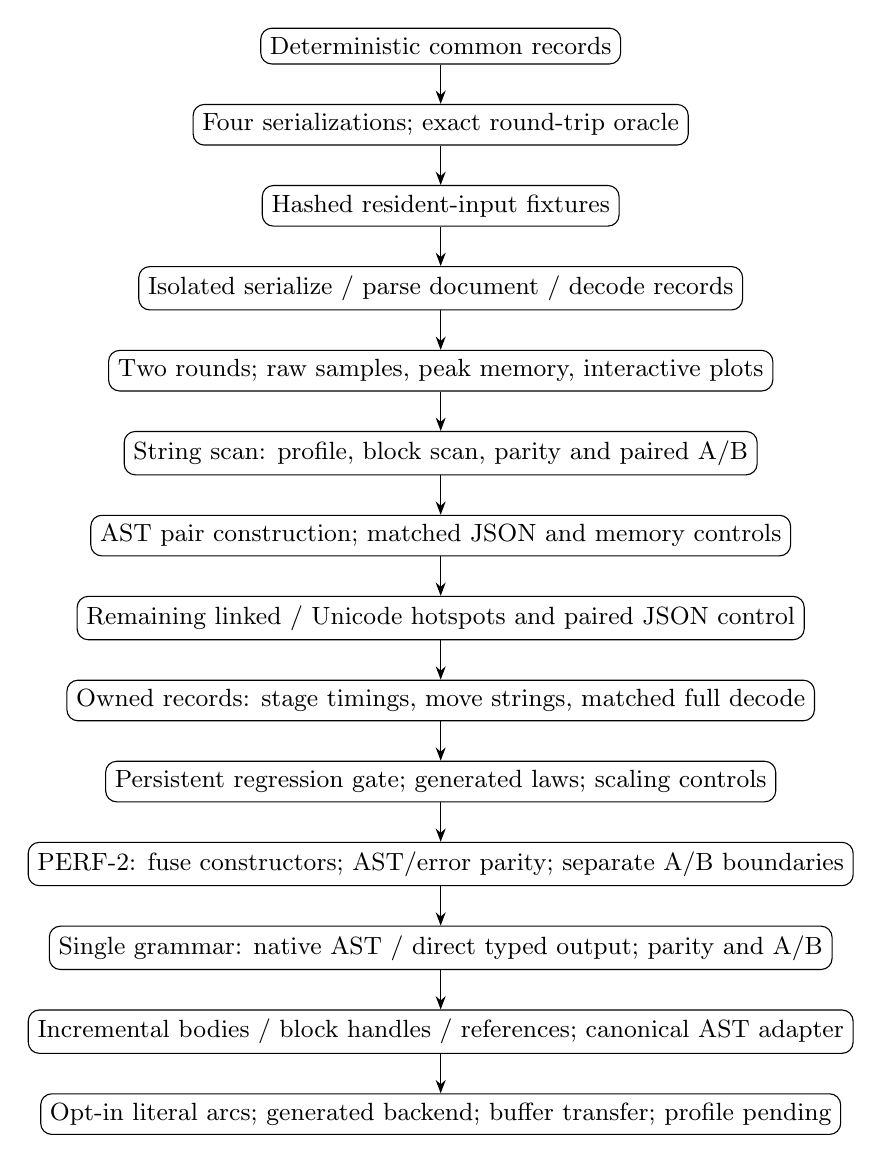
\begin{tikzpicture}[node distance=5mm,every node/.style={draw,rounded corners,font=\small},>=Stealth]
\node (g) {Deterministic common records};
\node (s) [below=of g] {Four serializations; exact round-trip oracle};
\node (f) [below=of s] {Hashed resident-input fixtures};
\node (p) [below=of f] {Isolated serialize / parse document / decode records};
\node (r) [below=of p] {Two rounds; raw samples, peak memory, interactive plots};
\draw[->] (g)--(s);\draw[->] (s)--(f);\draw[->] (f)--(p);\draw[->] (p)--(r);
\node (l) [below=of r] {String scan: profile, block scan, parity and paired A/B};
\draw[->] (r)--(l);
\node (a) [below=of l] {AST pair construction; matched JSON and memory controls};
\draw[->] (l)--(a);
\node (h) [below=of a] {Remaining linked / Unicode hotspots and paired JSON control};
\draw[->] (a)--(h);
\node (o) [below=of h] {Owned records: stage timings, move strings, matched full decode};
\draw[->] (h)--(o);
\node (q) [below=of o] {Persistent regression gate; generated laws; scaling controls};
\draw[->] (o)--(q);
\node (f2) [below=of q] {PERF-2: fuse constructors; AST/error parity; separate A/B boundaries};
\draw[->] (q)--(f2);
\node (b2) [below=of f2] {Single grammar: native AST / direct typed output; parity and A/B};
\draw[->] (f2)--(b2);
\node (c3) [below=of b2] {Incremental bodies / block handles / references; canonical AST adapter};
\draw[->] (b2)--(c3);
\node (f4) [below=of c3] {Opt-in literal arcs; generated backend; buffer transfer; profile pending};
\draw[->] (c3)--(f4);
\end{tikzpicture}

% 2026-09-08: Profile native AST; optimize proven hotspot; matched A/B preserves corpus.
\end{center}
\end{document}
